\begin{figure*}[p]
\centering

\newcommand{\codefile}[1]{%
    \lstinputlisting[
        style=mystyle,
        basicstyle=\fontsize{4.1}{4.5}\selectfont\ttfamily,
        frame=none,
        backgroundcolor=\color{white},
        aboveskip=1pt,
        belowskip=0pt,
        xleftmargin=1pt,
        xrightmargin=1pt
    ]{#1}%
}

\newcommand{\smalltitle}[1]{%
    {\fontsize{7}{7.5}\selectfont\bfseries #1}
}

\begin{tcolorbox}[
    width=\textwidth,
    colback=magenta!3,
    colframe=purple!40,
    title=Example with TikZ Code,
    enhanced,
    sharp corners=south,
    boxrule=0.5pt,
    left=2mm,
    right=2mm,
    top=1mm,
    bottom=1mm
]

\begin{minipage}[t]{0.29\linewidth}
\centering
\smalltitle{Source}

\vspace{1mm}

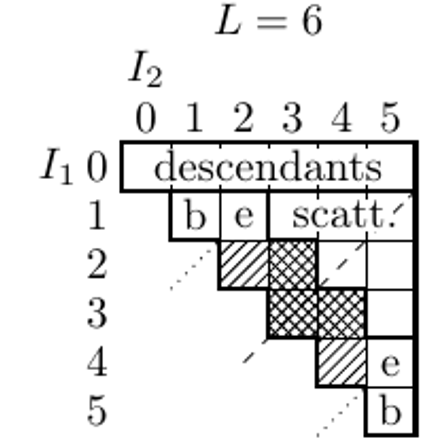
\includegraphics[
    width=\linewidth,
    height=2.9cm,
    keepaspectratio
]{structure/examples_new/sample_0604_source.png}
\end{minipage}
%
\hfill
%
\begin{minipage}[t]{0.36\linewidth}
\centering
\smalltitle{Edit Instruction}

\vspace{-2mm}

\begin{tcolorbox}[
    colback=white,
    colframe=gray!45,
    boxrule=0.3pt,
    arc=1mm,
    left=1mm,right=1mm,
    top=1mm,bottom=1mm
]
\raggedright
\fontsize{4.4}{5.1}\selectfont
      The grid structure is expanded from a 6x6 matrix to a 7x7 matrix, adding a new column (index 6) and a new row (index 6) to the axes and the grid lines. The text label 'e' located at grid position (2, 1) is changed to 'b'." The fill pattern of the cell at grid position (3, 2) is changed from crosshatch to diagonal lines (north east lines). The fill pattern of the cell at grid position (4, 4) is changed from diagonal lines (north east lines) to crosshatch. A new filled cell with diagonal lines (north east lines) pattern is added at grid position (5, 4). A new filled cell with diagonal lines (north east lines) pattern is added at grid position (5, 5). The text label 'e' located at grid position (5, 4) is changed to 'b'. A new text label 'b' is added at grid position (6, 5). The dashed line indicating the boundary of the 'scatt.' region is extended to accommodate the larger grid size, now ending at the bottom right corner of the 7x7 grid.
\end{tcolorbox}
\end{minipage}
%
\hfill
%
\begin{minipage}[t]{0.29\linewidth}
\centering
\smalltitle{Ground Truth}

\vspace{1mm}

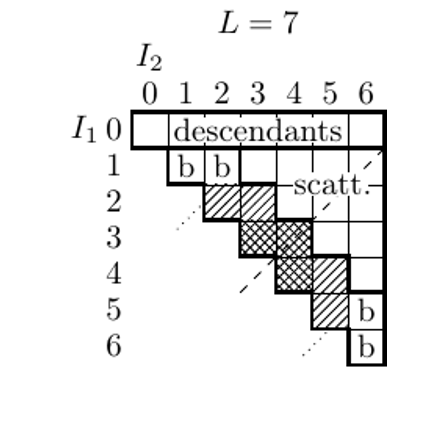
\includegraphics[
    width=\linewidth,
    height=2.9cm,
    keepaspectratio
]{structure/examples_new/sample_0604_gt.png}
\end{minipage}

\vspace{2mm}

\begin{minipage}[t]{0.44\linewidth}
\vspace{0pt}
\begin{tcolorbox}[
    width=\linewidth,
    colback=white,
    colframe=gray!45,
    boxrule=0.3pt,
    arc=1mm,
    left=0.5mm,right=0.5mm,
    top=0.5mm,bottom=0.5mm
]
\codefile{structure/examples_new/sample_0604_source.tex}
\end{tcolorbox}
\end{minipage}
%
\hfill
%
\begin{minipage}[t]{0.44\linewidth}
\vspace{0pt}
\begin{tcolorbox}[
    width=\linewidth,
    colback=white,
    colframe=gray!45,
    boxrule=0.3pt,
    arc=1mm,
    left=0.5mm,right=0.5mm,
    top=0.5mm,bottom=0.5mm
]
\codefile{structure/examples_new/sample_0604_gt.tex}
\end{tcolorbox}
\end{minipage}

\vspace{1mm}

\tcblower

\begin{minipage}[t]{0.485\linewidth}
\centering
\smalltitle{GPT-5.6-Sol}

\vspace{1mm}

\begin{tikzpicture}
\node[inner sep=0] (img) {%
    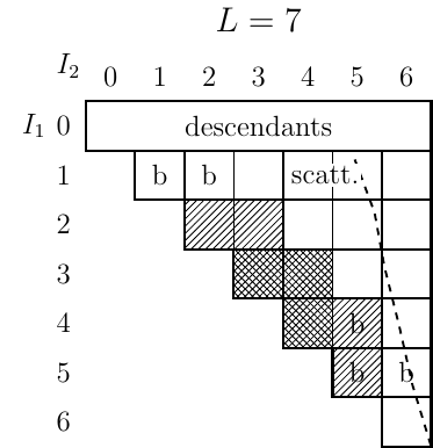
\includegraphics[
        width=0.72\linewidth,
        height=2.9cm,
        keepaspectratio
    ]{structure/examples_new/sample_0604_gpt.png}%
};

\node[
    anchor=west,
    right=1.5mm of img.east,
    align=left,
    fill=white,
    draw=gray!45,
    line width=0.3pt,
    rounded corners=1mm,
    inner xsep=1mm,
    inner ysep=0.8mm
] {%
    \fontsize{5.0}{5.8}\selectfont
    \begin{tabular}{@{}lr@{}}
    \textbf{TED}  & 0.647 \\
    \textbf{DSim} & 0.867 \\
    \textbf{EA}   & 0.500 \\
    \textbf{SP}   & 0.600 \\
    \textbf{VQ}   & 0.900 \\
    \textbf{AT}   & 671
    \end{tabular}
};
\end{tikzpicture}

\vspace{1mm}

\begin{tcolorbox}[
    colback=white,
    colframe=gray!45,
    boxrule=0.3pt,
    arc=1mm,
    left=0.5mm,right=0.5mm,
    top=0.5mm,bottom=0.5mm
]
\codefile{structure/examples_new/sample_0604_gpt.tex}
\end{tcolorbox}
\end{minipage}
%
\hfill
%
\begin{minipage}[t]{0.485\linewidth}
\centering
\smalltitle{EdiTikZ-4B-RL}

\vspace{1mm}

\begin{tikzpicture}
\node[inner sep=0] (img) {%
    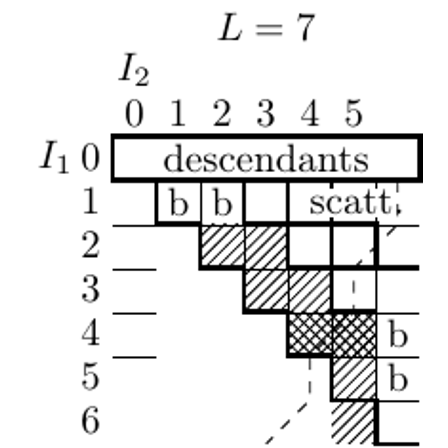
\includegraphics[
        width=\linewidth,
        height=2.9cm,
        keepaspectratio
    ]{structure/examples_new/sample_0604_4b_rl.png}%
};

\node[
    anchor=west,
    right=1.5mm of img.east,
    align=left,
    fill=white,
    draw=gray!45,
    line width=0.3pt,
    rounded corners=1mm,
    inner xsep=1mm,
    inner ysep=0.8mm
] {%
    \fontsize{5.0}{5.8}\selectfont
    \begin{tabular}{@{}lr@{}}
    \textbf{TED}  & 0.804 \\
    \textbf{DSim} & 0.938 \\
    \textbf{EA}   & 0.200 \\
    \textbf{SP}   & 0.200 \\
    \textbf{VQ}   & 0.400 \\
    \textbf{AT}   & 1209
    \end{tabular}
};
\end{tikzpicture}

\vspace{1mm}

\begin{tcolorbox}[
    colback=white,
    colframe=gray!45,
    boxrule=0.3pt,
    arc=1mm,
    left=0.5mm,right=0.5mm,
    top=0.5mm,bottom=0.5mm
]
\codefile{structure/examples_new/sample_0604_4b_rl.tex}
\end{tcolorbox}
\end{minipage}

\end{tcolorbox}

\caption{TikZ programs and rendered figures for a representative scientific-figure edit. Models receive the source figure and edit instruction and generate the edited TikZ program. Per-example TED, DSim, EA, SP, VQ, and AT are shown beside each prediction.}
\label{fig:tikz_code_example_2}

\end{figure*}